\chapter{Penrose Diagrams and the Formation of a Real Black Hole}

The Kruskal picture gives an elegant description of the neighborhood of a
Schwarzschild horizon, but a real black hole is not eternal: it forms when
matter collapses.  Which parts of the extended picture survive that physical
history?  To answer the question we need a diagram large enough to contain an
entire spacetime and disciplined enough to preserve the motion of light.  We
will first compactify flat spacetime, then compactify Schwarzschild spacetime,
and finally sew the appropriate pieces together across an infalling shell of
radiation.

\section{Near the Horizon: Kruskal Recap and the Four Quadrants}

We begin exactly where the previous lecture left off. Very near the Schwarzschild horizon, the geometry looks locally like flat space. The horizon itself behaves like a hyperbolic polar-coordinate locus, much as accelerated coordinates do in ordinary Minkowski spacetime. In this local picture we impose one rule from the start and never relax it: radial light rays are drawn at \(45^\circ\), and every timelike worldline must remain steeper than those null lines.

The coordinates in this recap are best thought of as time and space as seen by an infalling observer. In those locally inertial coordinates the neighborhood of the horizon looks almost flat. But an observer who insists on hovering at fixed radius outside the hole is not inertial. Relative to the infalling frame, such a person traces an accelerated curve. The closer one hovers to the horizon, the larger the acceleration needed to stay out. That is the physical content of the family of exterior curves drawn on the right-hand side of the board.

\begin{figure}[htbp]
\centering

\includegraphics[width=0.72\textwidth]{lecture_08_figure_02.png}
\caption{Board sketch of the four-region near-horizon geometry. The red curves in the exterior record a family of hovering worldlines at fixed radius.}
\lectureframe{00:02:54}
\end{figure}

\begin{figure}[htbp]
\centering
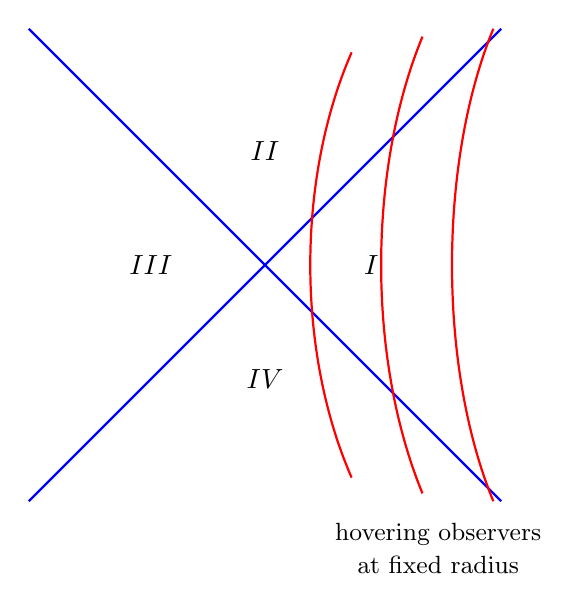
\begin{tikzpicture}[scale=1.0]
\draw[thick,blue] (-3,3) -- (3,-3);
\draw[thick,blue] (-3,-3) -- (3,3);

\draw[red,thick] (1.1,-2.7) .. controls (0.4,-1.1) and (0.4,1.1) .. (1.1,2.7);
\draw[red,thick] (2.0,-2.9) .. controls (1.3,-1.2) and (1.3,1.2) .. (2.0,2.9);
\draw[red,thick] (2.9,-3.0) .. controls (2.2,-1.3) and (2.2,1.3) .. (2.9,3.0);

\node at (1.35,0.0) {$I$};
\node at (0.0,1.45) {$II$};
\node at (-1.45,0.0) {$III$};
\node at (0.0,-1.45) {$IV$};

\node[align=center] at (2.2,-3.6) {\small hovering observers\\\small at fixed radius};
\end{tikzpicture}
\caption{Clean redraw of the Kruskal-style causal structure used in the recap. Region \(I\) is the exterior, region \(II\) the inescapable interior, and regions \(III\) and \(IV\) belong to the formal extension that will later be discarded for a real collapsing black hole.}
\end{figure}

This is already enough to say what a black hole does. In the exterior region \(I\), objects and signals may go inward, but they may also remain outside or turn back out. In region \(II\), by contrast, the causal verdict is fixed. Once one is in the interior, there is no future-directed causal path back to the exterior. To escape from region \(II\) into either outside region would require a trajectory shallower than \(45^\circ\) somewhere, and therefore faster than light. Every allowed future timelike trajectory ends on the singularity.

This opening recap is not merely repetition. It prepares the chapter's main theme. The Kruskal picture is useful, but not all of it is physically meaningful for a real black hole.

\begin{classroomqa}
\audiencequestion{What are the axes of the diagram, and whose fixed-position
worldlines are the red curves?}
\lecturerresponse{The axes are time and space in coordinates natural to a
freely falling observer.  Near the horizon that observer sees an almost
ordinary flat spacetime.  The red constant-position curves instead belong to
observers held stationary outside the hole.  They are accelerated worldlines,
with the required acceleration increasing toward the horizon.
\lecturetimestamp{00:05:58--00:06:47}}
\end{classroomqa}

\section{Why Compactify? From Infinite Spacetime to a Finite Blackboard}

The next move is methodological. The null directions in these diagrams run off to infinity, and so does time itself. We therefore cannot draw the whole spacetime on an ordinary blackboard unless we change coordinates. The lecturer's motivation is very concrete: if we want to see everything at once and reason about the global causal structure, we need a way to compress an infinite spacetime into a finite region while keeping light rays recognizable.

He therefore backs up to the easy case, good old flat spacetime. Because the problems of interest are spherically symmetric, we suppress the angular directions and keep only time and the radial coordinate. We use coordinates \(T\) and \(R\), with
\[
R\ge 0,
\]
since negative radial distance has no meaning in polar coordinates. We also choose units in which
\[
c=1.
\]
With that convention, radial null motion is drawn at \(45^\circ\).

Before introducing the compactifying map, the lecture takes some time to orient us in the \(T\)-\(R\) plane. One draws the time axis, the radial axis, a few constant-time slices \(T=0,\pm1,\pm2\), and a few constant-radius lines \(R=1,2,3\). This is not dead formalism. It gives us landmarks, and it makes clear which features we want to preserve when the diagram is later squeezed into finite size.

There is also a subtle but important pedagogical point about the origin. In the reduced radial picture, a light ray aimed exactly at \(R=0\) appears to bounce from the origin and come back out. But nothing is physically reflecting from a wall. In the full spherically symmetric geometry the ray simply passes through the origin and emerges on the other side. The apparent bounce is only a consequence of working with the half-plane \(R\ge 0\).

Likewise, a light ray that misses the origin starts by looking almost the same, reaches a point of closest approach, and then turns back outward. In these coordinates it may even look as if something has repelled it from the origin. But that too is a coordinate description of the familiar angular-momentum barrier, not a new force. The lecturer lingers over these examples because he wants the audience to trust the diagram before he deforms it.

Now comes the essential move. We are going to squeeze and stretch the picture, but keep one thing fixed: radial light rays must remain \(45^\circ\) lines. That is the whole point of the compactification.

\begin{classroomqa}
\audiencequestion{Is there anything physically special at the chosen origin,
and are the apparently bent rays evidence of a force there?}
\lecturerresponse{No.  At this stage the origin is merely the center selected
by spherical coordinates.  The apparent bounce and bending come from reducing
the full spatial motion to \(R\geq0\).  Symmetry may make a center convenient,
as it does for the Sun, but the coordinate choice does not put a black hole or
a reflecting wall there.
\lecturetimestamp{00:16:27--00:17:08}}
\end{classroomqa}

\section{Flat Spacetime in Null Coordinates and Penrose Form}

To make the deformation precise, we introduce null coordinates. This is the mathematically clean part of the lecture, and the board makes the move explicit.

\begin{figure}[htbp]
\centering

\includegraphics[width=0.82\textwidth]{lecture_08_figure_03.png}
\caption{The unobstructed \(T\)-\(R\) board at the introduction of
\(T^+=T+R\) and \(T^-=T-R\).  The reduced radial origin is the blue
vertical line \(R=0\).}
\lectureframe{00:19:45}
\end{figure}

We define
\begin{align}
T^+ &= T+R, \\
T^- &= T-R.
\end{align}
These are adapted to radial null motion. An ingoing radial light ray has \(T^+=\text{const}\), while an outgoing radial light ray has \(T^-=\text{const}\).

\paragraph{Worked derivation.}
The line \(R=0\) becomes particularly simple in these coordinates. Indeed,
\begin{align}
R=0
&\iff T+R=T-R \\
&\iff T^+=T^-.
\end{align}
So the entire timelike boundary \(R=0\) is described by the single relation
\begin{equation}
R=0 \iff T^+=T^-.
\end{equation}

\begin{figure}[htbp]
\centering
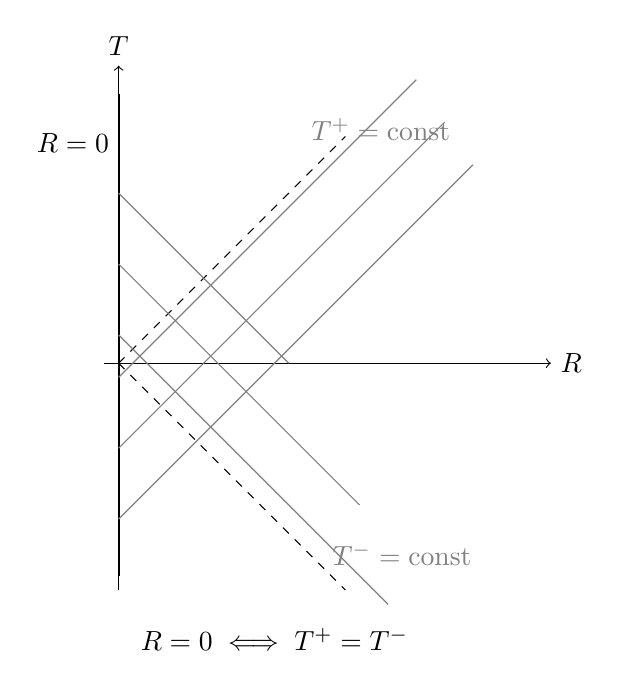
\begin{tikzpicture}[scale=0.9]
\draw[->] (-0.2,0) -- (6.1,0) node[right] {$R$};
\draw[->] (0,-3.2) -- (0,4.2) node[above] {$T$};

\draw[thick] (0,-3.0) -- (0,3.8);
\node[left] at (0,3.1) {$R=0$};

\draw[dashed] (0,0) -- (3.2,3.2);
\draw[dashed] (0,0) -- (3.2,-3.2);

\draw[gray] (0,2.4) -- (2.4,0);
\draw[gray] (0,1.4) -- (3.4,-2.0);
\draw[gray] (0,0.4) -- (3.8,-3.4);

\draw[gray] (0,-2.2) -- (5.0,2.8);
\draw[gray] (0,-1.2) -- (4.6,3.4);
\draw[gray] (0,-0.2) -- (4.2,4.0);

\node[gray] at (3.7,3.3) {$T^+=\mathrm{const}$};
\node[gray] at (4.0,-2.7) {$T^-=\mathrm{const}$};

\node at (2.2,-3.9) {$R=0 \iff T^+=T^-$};
\end{tikzpicture}
\caption{A clean \(T\)-\(R\) redraw. The two null families are the level sets of \(T^+\) and \(T^-\), and the line \(R=0\) is equivalently \(T^+=T^-\).}
\end{figure}

Now we compactify. We introduce two new null coordinates \(U^\pm\), each obtained from the corresponding \(T^\pm\) by the same bounded monotone function \(F\):
\begin{align}
U^+ &= F(T^+), &
U^- &= F(T^-),
\end{align}
with
\begin{equation}
F(+\infty)=1,
\qquad
F(-\infty)=-1.
\end{equation}
The lecture's convenient choice is
\begin{equation}
F(x)=\tanh x,
\end{equation}
so that
\begin{equation}
U^+ = \tanh(T^+),
\qquad
U^- = \tanh(T^-).
\end{equation}
There is nothing sacred about the hyperbolic tangent. It is simply a smooth function with the right limiting behavior, and so it squeezes infinite coordinate ranges down to finite ones.

The null structure is preserved for a simple reason. If an ingoing radial light ray has \(T^+=\text{const}\), then
\[
U^+=F(T^+)=\text{const},
\]
and similarly if an outgoing radial light ray has \(T^-=\text{const}\), then
\[
U^-=F(T^-)=\text{const}.
\]
Thus the compactification separately reparametrizes the two null directions, and radial light rays remain \(45^\circ\) lines. The origin line is carried along just as cleanly:
\[
T^+=T^- \Longrightarrow U^+=U^-.
\]

At this point the infinite half-plane of flat spacetime has been compressed to a finite triangle. The lecture then teaches us how to read its edges. Spatial infinity collapses to a single point \(i^0\). Future and past timelike infinities are \(i^+\) and \(i^-\). The two null edges are \(\mathcal{I}^+\) and \(\mathcal{I}^-\), often pronounced scri-plus and scri-minus, the places where incoming and outgoing light rays begin and end.

\begin{figure}[htbp]
\centering
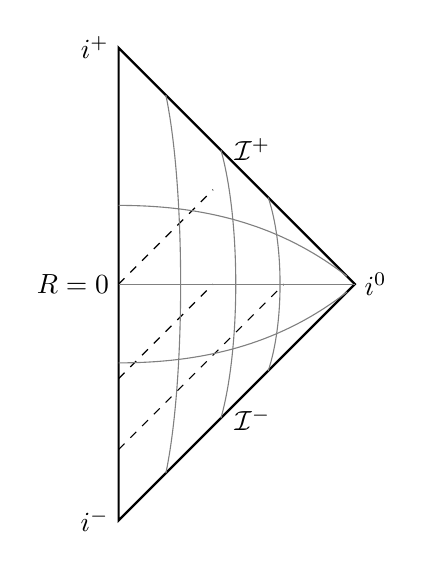
\begin{tikzpicture}[scale=1.0]
\draw[thick] (0,-3) -- (0,3) -- (3,0) -- cycle;

\node[left] at (0,3) {$i^+$};
\node[left] at (0,-3) {$i^-$};
\node[right] at (3,0) {$i^0$};
\node[left] at (0,0) {$R=0$};
\node[above right] at (1.35,1.45) {$\mathcal{I}^+$};
\node[below right] at (1.35,-1.45) {$\mathcal{I}^-$};

\draw[dashed] (0,-2.1) -- (2.1,0.0);
\draw[dashed] (0,-1.2) -- (1.2,0.0);
\draw[dashed] (0,0.0) -- (1.2,1.2);

\draw[gray] (0,0) -- (3,0);
\draw[gray] (0,1.0) .. controls (1.0,1.0) and (2.0,0.8) .. (2.9,0.1);
\draw[gray] (0,-1.0) .. controls (1.0,-1.0) and (2.0,-0.8) .. (2.9,-0.1);

\draw[gray] (0.6,-2.4) .. controls (0.85,-1.2) and (0.85,1.2) .. (0.6,2.4);
\draw[gray] (1.3,-1.7) .. controls (1.55,-0.8) and (1.55,0.8) .. (1.3,1.7);
\draw[gray] (1.9,-1.1) .. controls (2.1,-0.5) and (2.1,0.5) .. (1.9,1.1);
\end{tikzpicture}
\caption{Penrose diagram for radially reduced flat spacetime. Constant-time curves run outward toward \(i^0\), while constant-radius curves rise from \(i^-\) toward \(i^+\).}
\end{figure}

One last point from the lecture should be kept in mind. These diagrams do \emph{not} preserve metric size. They preserve causal structure. That is the invariant we are after.

\begin{classroomqa}
\audiencequestion{Are the compactified constant-time lines supposed to be
straight?}
\lecturerresponse{Only the symmetric slice \(T=0\) is straight for the
chosen map.  The other constant-\(T\) curves bend, and their detailed shapes
depend on the compactifying function.  Very late slices crowd ever closer to
the upper boundary even though ordinary time continues without bound.
\lecturetimestamp{00:29:11--00:30:12}}
\end{classroomqa}

\section{The Compactified Schwarzschild Geometry}

Armed with the flat-space construction, we now return to the black hole and do the same thing again. We compactify the Kruskal geometry by introducing null coordinates and squeezing the infinite ranges into a finite figure. The lecturer describes the result as a diagonal rectangle or diamond-like causal picture: the horizon appears as a null boundary, the exterior hovering worldlines stay outside it, and the interior region terminates on a singularity that is now visible on the page.

The crucial physical point is that the singularity is \emph{not} at infinity in the infalling observer's experience. Once the horizon is crossed, the remaining proper time before striking the singularity is finite. The Penrose diagram makes this visually unavoidable.

The horizon is again identified by the Schwarzschild condition
\begin{equation}
1-\frac{2MG}{r}=0
\qquad \Longleftrightarrow \qquad
r=2MG.
\end{equation}
The equality \(r=2MG\) marks the radius where the Schwarzschild factor
changes sign.

\begin{figure}[htbp]
\centering

\includegraphics[width=0.72\textwidth]{lecture_08_figure_04.png}
\caption{Board sketch contrasting the formal extended picture with the physically relevant black-hole region. The red label \emph{singularity} is explicit on the board.}
\lectureframe{00:37:59}
\end{figure}

\begin{figure}[htbp]
\centering
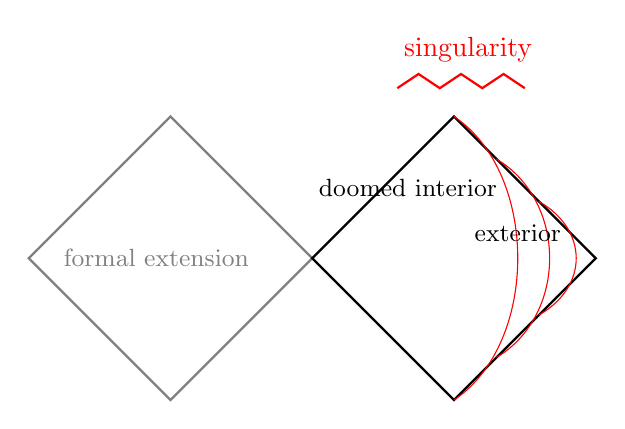
\begin{tikzpicture}[scale=0.9]
\draw[gray,thick] (-4,0) -- (-2,2) -- (0,0) -- (-2,-2) -- cycle;
\draw[thick] (0,0) -- (2,2) -- (4,0) -- (2,-2) -- cycle;

\draw[red,thick] (1.2,2.4) -- (1.5,2.6) -- (1.8,2.4) -- (2.1,2.6) -- (2.4,2.4) -- (2.7,2.6) -- (3.0,2.4);
\node[red] at (2.2,2.95) {singularity};

\draw[red] (2.0,-2.0) .. controls (3.2,-1.2) and (3.2,1.2) .. (2.0,2.0);
\draw[red] (2.6,-1.4) .. controls (3.6,-0.8) and (3.6,0.8) .. (2.6,1.4);
\draw[red] (3.2,-0.8) .. controls (3.9,-0.4) and (3.9,0.4) .. (3.2,0.8);

\node at (2.9,0.35) {\small exterior};
\node at (1.35,1.0) {\small doomed interior};
\node[gray] at (-2.2,0.0) {\small formal extension};
\end{tikzpicture}
\caption{A conservative redraw of the causal picture emphasized in the lecture: the surviving exterior, the doomed interior, the future singularity, and the contrast with the extra formal part of the extension.}
\end{figure}

The lecture is very direct here. If you are in the exterior, you may still escape, or you may fall in. If you are in the interior, you are doomed. The diagram is already saying everything important about future-directed causal motion.

Quadrants \(III\) and \(IV\) are legitimate parts of the maximally extended
Kruskal solution.  Region \(III\) supplies a second exterior, and region \(IV\)
is the time-reversed black-hole region.  They do not, however, occur in the
spacetime of an ordinary black hole made by collapse.  The extended solution
is mathematically instructive precisely because the collapse construction
will show us which pieces must be discarded.

\section{Spatial Slices, Two-Spheres, and the Einstein--Rosen Bridge}

Now freeze the compactified diagram on a spacelike slice and ask what that
slice looks like as \emph{space} rather than spacetime.  This is where the
wormhole image enters, and where the spatial picture must not be allowed to
outrun the causal argument.

Because the angular directions have been suppressed, each point of the
radial diagram represents a two-sphere. At Schwarzschild radius \(r\), its
area is
\begin{equation}
A=4\pi r^2.
\end{equation}
A spacelike slice is therefore a family of two-spheres, not merely a
one-dimensional curve. Their size changes as one moves along the slice.

Far away the spheres are very large. As one moves inward, their radius shrinks until it reaches a minimum at the horizon,
\begin{equation}
r_{\min}=2MG.
\end{equation}
If one keeps going through the formal extension, the spheres expand again toward another asymptotic side. This is the Einstein--Rosen bridge picture.

\begin{figure}[htbp]
\centering

\includegraphics[width=0.72\textwidth]{lecture_08_figure_05.png}
\caption{The extended Kruskal diagram with the green spacelike slice used to
construct the bridge geometry.  Every point on that slice represents a
two-sphere; its minimum radius is marked \(r=2MG\).}
\lectureframe{00:41:30}
\end{figure}

The board shows only part of the relevant Schwarzschild factor,
\begin{equation}
1-\frac{2MG}{r},
\end{equation}
and the throat occurs at the same special radius \(r=2MG\).

\begin{figure}[htbp]
\centering
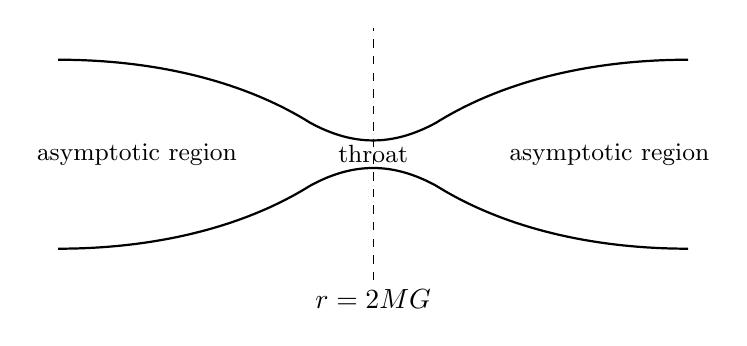
\begin{tikzpicture}[scale=1.0]
\draw[thick] (-4,1.2)
.. controls (-2.7,1.2) and (-1.6,0.9) .. (-0.8,0.4)
.. controls (-0.25,0.1) and (0.25,0.1) .. (0.8,0.4)
.. controls (1.6,0.9) and (2.7,1.2) .. (4,1.2);

\draw[thick] (-4,-1.2)
.. controls (-2.7,-1.2) and (-1.6,-0.9) .. (-0.8,-0.4)
.. controls (-0.25,-0.1) and (0.25,-0.1) .. (0.8,-0.4)
.. controls (1.6,-0.9) and (2.7,-1.2) .. (4,-1.2);

\draw[dashed] (0,-1.6) -- (0,1.6);
\node[below] at (0,-1.6) {$r=2MG$};
\node at (0,0) {\small throat};
\node at (-3.0,0) {\small asymptotic region};
\node at (3.0,0) {\small asymptotic region};
\end{tikzpicture}
\caption{Schematic spatial slice through the extended Schwarzschild geometry. This is a cautious reconstruction of the lecture's bridge picture, not a literal embedding calculation.}
\end{figure}

Now comes the correction. The slice suggests a bridge between two asymptotic regions, and so it invites the thought that one might travel from one universe to the other by passing through the neck. The lecture first lets that suggestion appear, and then kills it causally. To get from one exterior region to the other, a worldline would have to become shallower than a \(45^\circ\) null line somewhere on the Penrose diagram. That is forbidden. So the Einstein--Rosen bridge is non-traversable.

The lecturer also emphasizes why the spatial picture can mislead. It is a picture of \emph{space at an instant of time}; but there is simply not enough causal time to get through. One can say, loosely, that the bridge opens and closes before anything can cross it. Better still, one simply looks back at the Penrose diagram and reads off the causal answer.

\section{Building a Real Black Hole from an Infalling Null Shell}

At this point the lecture changes problem completely. We are no longer reading off the properties of an eternal black hole. We are constructing a real one.

The model is chosen for simplicity. We imagine not a collapsing star with messy internal structure, but a thin spherical shell of incoming radiation. It is a shell of light, and therefore moves inward at the speed of light. At sufficiently small radius the energy on that shell is concentrated tightly enough that a black hole forms.

The second ingredient is the shell theorem in its general-relativistic form.

\paragraph{Remark.} For the spherically symmetric shell used in this lecture, the interior region is flat spacetime, while the exterior region is Schwarzschild. This is the operational shell theorem, or Birkhoff-type statement, used by the lecture. It is not proved here.

The lecturer motivates this by first recalling the Newtonian shell theorem: inside a spherical shell there is no gravitational field, while outside the shell the field is the same as that of a point mass at the center. He then states the corresponding relativistic version in the only form needed here: the inside is flat, the outside is Schwarzschild. The shell may move; the rule is the same.

That is enough to construct the collapse spacetime. The shell itself is null, so it must be drawn at \(45^\circ\). On one side of that null line the geometry is flat. On the other side it is Schwarzschild. We can summarize the rule as
\begin{equation}
\begin{aligned}
\text{inside shell} &= \text{flat spacetime},\\
\text{outside shell} &= \text{Schwarzschild geometry}.
\end{aligned}
\end{equation}

The gluing prescription then becomes almost embarrassingly simple:

\begin{enumerate}
\item Draw the flat Penrose diagram and keep only the region interior to the incoming shell.
\item Draw the Schwarzschild Penrose diagram and keep only the region exterior to that same shell.
\item Throw away the wrong pieces.
\item Sew the two surviving pieces together along the shell trajectory.
\end{enumerate}

This is exactly how the lecture proceeds on the board: discard the wrong half of one picture, discard the wrong half of the other, and glue the right halves along the shell.

\begin{figure}[htbp]
\centering
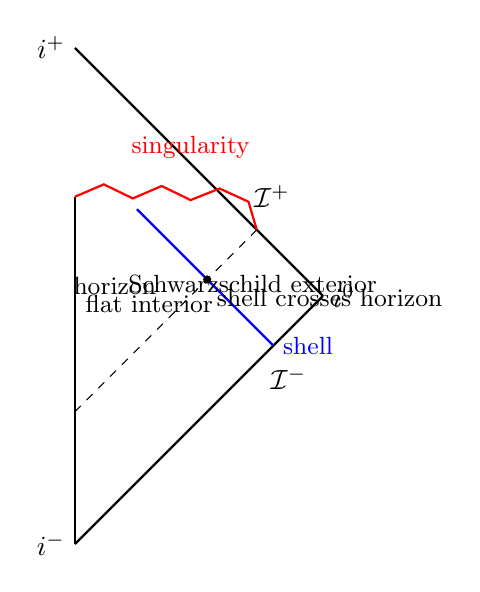
\begin{tikzpicture}[scale=1.05]
\coordinate (im) at (0,-3.0);
\coordinate (ip) at (0,3.0);
\coordinate (i0) at (3.0,0.0);
\coordinate (S)  at (0,1.2);
\coordinate (E)  at (2.2,0.8);
\coordinate (P)  at (2.4,-0.6);
\coordinate (Q)  at (0.75,1.05);
\coordinate (H)  at (0,-1.4);
\coordinate (X)  at (1.6,0.2);

\draw[thick] (im) -- (S);
\draw[thick] (im) -- (i0);
\draw[thick] (ip) -- (i0);

\draw[red,thick] (S) -- (0.35,1.35) -- (0.7,1.18) -- (1.05,1.33) -- (1.4,1.16) -- (1.75,1.30) -- (2.1,1.14) -- (E);
\node[red,above] at (1.4,1.55) {\small singularity};

\draw[thick,blue] (P) -- (Q);
\node[blue,right] at (P) {\small shell};

\draw[dashed] (H) -- (E);
\node[above left] at (1.1,-0.1) {\small horizon};

\filldraw (X) circle (1.2pt);
\node[below right] at (X) {\small shell crosses horizon};

\node at (0.9,-0.1) {\small flat interior};
\node at (2.15,0.15) {\small Schwarzschild exterior};

\node[left] at (im) {$i^-$};
\node[left] at (ip) {$i^+$};
\node[right] at (i0) {$i^0$};
\node[below right] at (2.25,-0.75) {$\mathcal{I}^-$};
\node[above right] at (2.05,0.95) {$\mathcal{I}^+$};
\end{tikzpicture}
\caption{Causal reconstruction of the collapse geometry. The shell is an ingoing null line; flat spacetime is kept on its interior side and Schwarzschild geometry on its exterior side.}
\end{figure}

\begin{figure}[htbp]
\centering

\includegraphics[width=0.76\textwidth]{lecture_08_figure_06.png}
\caption{The completed board construction after the flat interior and
Schwarzschild exterior have been glued along the blue infalling shell.  The
dashed \(45^\circ\) line is being traced backward from the future endpoint of
the singularity to locate the event horizon.}
\lectureframe{00:57:30}
\end{figure}

The shell itself experiences nothing special at the moment when it is merely crossing from the flat part of the diagram into the Schwarzschild part. It is a lightlike shell, and it continues inward until it reaches the singularity. The essential structure is not carried by local drama on the shell; it is carried by the causal organization of the glued spacetime.

\begin{classroomqa}
\audiencequestion{Is there a discontinuity when the collapsing shell crosses
its Schwarzschild radius?}
\lecturerresponse{No.  Nothing locally singular happens at that crossing.
The shell continues on its null trajectory.  The special event is causal:
after the shell has crossed its own \(2MG\) radius, no future-directed path
can return it to infinity.
\lecturetimestamp{00:56:19--00:56:42}}
\end{classroomqa}

\section{Horizon Before Arrival: The Event-Horizon Puzzle}

Now comes the conceptual climax of the lecture. Once the collapse spacetime has been built, the natural question is: where is the horizon? Or, as the lecturer puts it, where is the point of no return?

\paragraph{Definition.} The event horizon is the boundary between those events that can still send a future-directed causal signal to \(\mathcal{I}^+\) and those that cannot.

The lecture finds it diagrammatically. Start at the corner where the singularity meets future null infinity, and trace a \(45^\circ\) null line backward. That backward-traced null line is the event horizon.

But the lecturer then insists on a second point, and it is the one that makes students uneasy. The horizon does not simply appear at the moment when the shell crosses its own Schwarzschild radius and then stay put. In the enlarged board drawing, the horizon begins as a tiny trapped region near the center, expands outward through a part of spacetime that is still flat, and only later meets the incoming shell. At that meeting event the shell passes its own Schwarzschild radius. Above that event, the horizon is the ordinary constant-radius horizon of the completed black hole.

\begin{figure}[htbp]
\centering
\resizebox{0.96\linewidth}{!}{%
\begin{tikzpicture}[scale=1.08,>=Latex]
\coordinate (im) at (0,-3.0);
\coordinate (ip) at (0,3.0);
\coordinate (i0) at (3.0,0.0);
\coordinate (S)  at (0,1.2);
\coordinate (E)  at (2.2,0.8);
\coordinate (P)  at (2.4,-0.6);
\coordinate (Q)  at (0.75,1.05);
\coordinate (H)  at (0,-1.4);
\coordinate (X)  at (1.6,0.2);

\draw[thick] (im) -- (S);
\draw[thick] (im) -- (i0);
\draw[thick] (ip) -- (i0);

\draw[red,thick] (S) -- (0.35,1.35) -- (0.7,1.18) -- (1.05,1.33) -- (1.4,1.16) -- (1.75,1.30) -- (2.1,1.14) -- (E);
\node[red,above left] at (S) {\small singularity};

\draw[very thick,red] (H) -- (E);

\draw[thick,blue] (P) -- (Q);

\filldraw (X) circle (1.2pt);

\draw[gray] (0.0,-2.1) .. controls (0.85,-1.95) and (1.9,-1.3) .. (2.8,-0.2);
\draw[gray] (0.0,-1.2) .. controls (0.95,-1.0) and (1.8,-0.45) .. (2.45,0.35);
\draw[gray] (0.0,-0.2) .. controls (0.8,-0.05) and (1.45,0.35) .. (1.95,0.95);

\node[below right] at (2.28,-0.72) {$\mathcal{I}^-$};
\node[above right] at (2.12,0.92) {$\mathcal{I}^+$};

\draw[very thick,red] (3.2,-1.15) -- (3.75,-1.15);
\node[anchor=west] at (3.85,-1.15) {\small event horizon};
\draw[thick,blue] (3.2,-1.55) -- (3.75,-1.55);
\node[anchor=west] at (3.85,-1.55) {\small infalling shell};
\filldraw (3.48,-1.95) circle (1.2pt);
\node[anchor=west] at (3.85,-1.95)
  {\small shell reaches \(r=2MG\)};
\end{tikzpicture}
}
\caption{The collapse diagram with the backward-traced event horizon emphasized. Part of the horizon lies in a region that is still locally flat and has not yet been reached by the shell.}
\end{figure}

This is the striking effect on which the rest of the lecture dwells.  Part of
the horizon lies in flat spacetime.  The shell has not yet arrived there, and
it is not even visible on the observer's past light cone.  The observer feels
no gravitational field and nevertheless cannot escape.  The reason is not a
local force.  It is the global causal future of the event.

\begin{classroomqa}
\audiencequestion{Does the construction say that one cannot cross the shell,
or that one cannot cross the horizon?  Where is the shell when its horizon is
still inside it?}
\lecturerresponse{One can cross the shell.  The horizon is a different null
surface: it is the boundary between events that can communicate with
\(\mathcal I^+\) and events that cannot.  The incoming shell meets that
boundary precisely when it crosses the Schwarzschild radius associated with
its total energy.  Before the meeting, part of the event horizon runs through
the flat interior; after the meeting, the shell lies inside the finished
black hole.
\lecturetimestamp{00:58:42--01:01:06}}
\end{classroomqa}

\begin{classroomqa}
\audiencequestion{If the interior is flat and the shell is still far away,
why can someone just inside the horizon not walk across it before the shell
arrives?}
\lecturerresponse{Draw the fastest possible outward worldline, a \(45^\circ\)
light ray.  From an event inside the backward-traced horizon even that ray
meets the incoming shell too late and ends at the singularity.  Walking is
slower still.  The phrase \emph{the shell has not crossed yet} is incomplete
until a time coordinate has been chosen; the causal diagram supplies the
coordinate-independent answer.  The incoming cosmic microwave background is
not the same example, because it is not a collapsing spherical shell that
creates this geometry.
\lecturetimestamp{01:01:07--01:04:03}}
\end{classroomqa}

\section{Mirrors and Attempts to Change the Future}

The questions now turn the diagram into a laboratory.  Suppose an incoming
light shell could be reflected before it became trapped.  Then the assumed
collapse history would change, and so would the event horizon.  This is not a
contradiction: an event horizon is defined only after the complete spacetime
history has been specified.

\begin{classroomqa}
\audiencequestion{What if a perfectly reflecting mirror is placed just
outside the would-be Schwarzschild radius so that the shell bounces back out?}
\lecturerresponse{In that idealized history the incoming null line turns
outward at the mirror and reaches the future boundary; the black hole in the
original diagram does not form.  A truly weightless mirror is impossible, and
a physical mirror contributes stress-energy of its own, but the thought
experiment makes the logical point: only after the shell crosses the actual
event horizon is escape no longer possible.
\lecturetimestamp{01:04:33--01:05:54}}
\end{classroomqa}

\begin{classroomqa}
\audiencequestion{Could an observer who knows the shell is coming quickly send
out a mirror or signal to make it turn around?}
\lecturerresponse{Only if the necessary apparatus can be placed outside the
horizon early enough.  Alice may arrange in advance for Bob to send the shell
and may therefore know what is coming before she sees it.  Once her event is
inside the horizon, however, neither a mirror nor an instruction can reach the
required exterior point in time.  Knowledge of the future experiment does not
open a causal path that the diagram forbids.
\lecturetimestamp{01:05:55--01:08:18}}
\end{classroomqa}

\begin{classroomqa}
\audiencequestion{What happens to a mirror already inside the horizon, and is
the singularity infinitely far in its future?}
\lecturerresponse{The mirror is simply another doomed object.  It may reflect
the light locally, but the reflected light, the mirror, and Alice all end on
the singularity.  A generic infalling worldline reaches it in finite proper
time.  Only the ideal upper corner of the compactified diagram is infinitely
far away.  Trying to remain near that corner would require unbounded
acceleration and energy; moreover, between fixed events an accelerated clock
accumulates less proper time than an inertial one, not more.
\lecturetimestamp{01:08:19--01:10:19}}
\end{classroomqa}

\begin{classroomqa}
\audiencequestion{If the collapsing shell is enormous, can someone inside the
shell but far from its eventual center simply remain there while it passes?}
\lecturerresponse{Yes, provided that person's event is still outside the
event horizon.  Being inside the material shell is not the same as being
inside the black hole.  The radiation may strike and injure the observer, but
that is a local interaction with the shell and is separate from the causal
question of escape.
\lecturetimestamp{01:10:21--01:11:24}}
\end{classroomqa}

\section{Time Slices and the Growing Horizon}

An \emph{instant of time} in curved spacetime means a chosen spacelike
hypersurface.  A stack of such surfaces is a foliation, and assigning a number
to each surface defines a time coordinate.  Different foliations cut the same
collapse diagram differently.  They disagree about which distant events are
simultaneous, but they do not change which null rays reach infinity.

\begin{figure}[htbp]
\centering

\includegraphics[width=0.77\textwidth]{lecture_08_figure_07.png}
\caption{The late board diagram with several green spacelike slices.  The
slices provide a time coordinate; the black null boundaries and their causal
relations are independent of that choice.}
\lectureframe{01:17:30}
\end{figure}

\begin{classroomqa}
\audiencequestion{Can the puzzle be restated by comparing, at one instant, the
distance from the observer to the horizon with the distance from the horizon
to the shell?}
\lecturerresponse{It can be a useful intuition after a foliation has been
chosen, but the phrase \emph{at one instant} is coordinate dependent.  The
clean construction is to draw a family of spacelike slices.  Early slices
meet a large shell and no trapped central region; later slices meet the
growing horizon inside the still-infalling shell; one distinguished slice
passes through the event where the shell crosses its own Schwarzschild
radius.
\lecturetimestamp{01:11:26--01:14:21}}
\end{classroomqa}

\begin{classroomqa}
\audiencequestion{Does the Schwarzschild radius grow as the horizon opens
outward, and why does the horizon keep growing after the shell crosses it?}
\lecturerresponse{The final Schwarzschild radius \(2MG\) is fixed because the
total mass \(M\) is fixed.  What grows on the early spacelike slices is the
areal radius of the horizon's cross-section.  It starts at the center,
increases until it meets the shell at \(r=2MG\), and then stops.  Above the
meeting event the horizon is the constant-\(r\) line \(r=2MG\), even though
compactification does not make that line look vertical or metrically
uniform.
\lecturetimestamp{01:14:22--01:16:15}}
\end{classroomqa}

\begin{classroomqa}
\audiencequestion{What happens to an observer initially at half the final
Schwarzschild radius?  Should that observer not feel gravity only when the
shell arrives?}
\lecturerresponse{Exactly.  The observer first crosses the growing event
horizon while still in flat spacetime and feels no sudden force.  The
infalling radiation shell is material and may later be felt; the event horizon
is not.  Crossing it means only that every future-directed causal path now
fails to reach infinity.  In that precise sense the horizon is ghostly.
\lecturetimestamp{01:16:17--01:17:45}}
\end{classroomqa}

\begin{classroomqa}
\audiencequestion{Can an observer who starts early enough move outward faster
than the growing horizon and escape?}
\lecturerresponse{Yes.  Events outside the horizon have outgoing causal paths
to \(\mathcal I^+\); events inside do not.  On a chosen slice one may compare
the available radial distance with the time before the incoming shell closes
the route, but the null lines give the exact test.  No observer sees a
material horizon rushing outward, because there is no local surface to see.
\lecturetimestamp{01:17:46--01:18:54}}
\end{classroomqa}

\section{What the Diagram Preserves}

The shapes on the page must not be read as a scale drawing.  A small corner
may represent an infinite region of spacetime, while a large patch may
represent a modest physical interval.  Compactification deliberately
sacrifices metric size in order to preserve null directions.  What survives
is cause and effect: who can send a signal to whom, which events can influence
which others, and which worldlines are trapped by the speed-of-light limit.

\begin{classroomqa}
\audiencequestion{If the picture distorts lengths and times so severely, what
does it represent faithfully?}
\lecturerresponse{It represents light rays and therefore causal structure.
To locate the event horizon, trace the last outgoing null ray backward from
future infinity.  Trying to infer the answer from apparent distances on the
page is unreliable.  Once the causal diagram is drawn, questions about
signals, escape, and no-return have geometric answers even though the metric
scale has been suppressed.
\lecturetimestamp{01:18:56--01:21:45}}
\end{classroomqa}

\begin{classroomqa}
\audiencequestion{How long does it take to become comfortable enough with
Penrose diagrams to use them intuitively?}
\lecturerresponse{Not long.  The practical prescription is to draw them,
trace null lines, and test possible worldlines until the causal restrictions
become familiar.  Intuition here is acquired by working with the diagrams,
not by guessing without them.
\lecturetimestamp{01:21:49--01:22:05}}
\end{classroomqa}

\begin{classroomqa}
\audiencequestion{Is this visual method the opposite of quantum mechanics,
where the mathematics is often more reliable than a picture?}
\lecturerresponse{To a considerable extent, yes.  General relativity is
classical physics.  Four-dimensional curved spacetime is difficult to picture
literally, and a Penrose diagram is still abstract, but its causal geometry
can be drawn and explored much further than the underlying reality of quantum
mechanics can.  That difference is part of what makes these diagrams so
powerful.
\lecturetimestamp{01:22:05--01:22:58}}
\end{classroomqa}
